\counterwithout{figure}{chapter}
\counterwithout{equation}{chapter}
%\chapter{Résumé étendu en français}\markboth{\sectionfont\itshape\color{activeColor}Résumé étendu en français}{} %%% IN FRONTMATTER
%\chapter{Résumé étendu en français} %%% IN MAINMATTER
\chapter{Résumé étendu en français}\fancyhead[RE,LO]{\subsectionfont\itshape\color{activeColor}Résumé étendu en français} %%% IN BACKMATTER
	\lettrine[lines=4]{\color{activeColor}D}{ans} cette thèse, nous étudions deux aspects de la dynamique des impuretés atomiques interagissant avec des nanogouttelettes d'hélium superfluide (He), à savoir la photo-excitation des alcalis sur une nanogouttelette et le dopage des nanogouttelettes contenant des tourbillons quantifiés avec des atomes de gaz rares. Pour les investigations théoriques, nous utilisons la théorie fonctionnelle He densité (He-DFT) et sa version dépendant du temps (He-TDDFT).

	Le premier aspect implique une collaboration expérimentale et théorique commune qui se concentre sur la photo-excitation du rubidium alcalin (Rb). Les alcalis sont une sonde très intéressante des gouttelettes d'He car elles résident dans leur région de surface, où l'on a avancé que près de 100\% de condensation de Bose-Einstein pouvait être obtenue en raison d'une densité inférieure à celle du He superfluide.
	
	Le deuxième aspect concerne une investigation purement théorique inspirée des travaux récents de Gomez et Vilesov \emph{et al}., où les tourbillons quantifiés ont été visualisés en dopant des nanoparticules d'He avec des atomes d'argent, puis en les \guillemotleft~soft landing~\guillemotright{} sur un écran carbone. Les images au microscope électronique montrent de longs filaments d'amas d'atomes d'argent qui s'accumulent le long des noyaux des vortex. La formation de réseaux de tourbillons quantiques à l'intérieur de nanogouttelettes est également mise en évidence en utilisant l'imagerie par diffraction des rayons~X pour visualiser les motifs de Bragg caractéristiques des amas de xénon (Xe) piégés à l'intérieur des noyaux de vortex.
	
	Nos simulations impliquant des gouttelettes hébergeant des tourbillons quantiques ouvrent la voie à d'autres investigations sur des gouttelettes hébergeant une série de vortex, impliquant de multiples impuretés.
		
	\section*{Introduction\\\small(Chapitre~1)}
		Jusqu'aux années 1980, la plupart des travaux expérimentaux et théoriques ont été effectués sur des systèmes en masse, c'est-à-dire des systèmes de l'ordre du nombre d'atomes $N_A$. Ce n'est qu'au cours des deux dernières décennies que les progrès technologiques ont permis aux expérimentateurs de créer des gouttelettes d'hélium superfluides de taille nanométrique. Dès le début des années 1990, les nanogouttelettes d'hélium superfluides sont devenues un champ d'étude actif, à la fois expérimentalement et théoriquement. 
		
		Les nanogouttelettes d'hélium sont considérées comme des systèmes modèles idéaux pour explorer l'hydrodynamique quantique dans des superfluides autonome et isolés. L'objectif principal a été l'évolution de leurs propriétés avec le nombre d'atomes dans le groupe, jusqu'à ce que la limite de matière condensée soit atteinte. Les amas d'hélium sont particulièrement intéressants dans la mesure où les effets quantiques jouent un rôle clé dans la détermination de leurs propriétés. En particulier, étant donné qu'un cluster d'hélium est un ensemble de bosons à environ 0.4~K\citep{Brink1990, Hartmann1995}, des manifestations de comportement collectif (comme la superfluidité) sont attendues. D'autre part, il n'est pas encore clair comment la taille finie d'un cluster affecte ce comportement collectif non-classique (ou dégénéré).

		Récemment, Toennies \emph{et al}. ont mesuré le spectre électronique de molécules de glyoxal noyées dans des amas d'He\citep{Hartmann1996} et l'ont trouvé cohérent avec une simulation théorique calculée en utilisant la courbe de dispersion de phonons d'He II en vrac superfluide. Les auteurs eux-mêmes soulignent cependant qu'à la taille moyenne des clusters de 5500 atomes d'He rapportée dans\rf{Hartmann1996}, les groupes sont si grands que les effets de taille finie dans la région intérieure sont négligeables (voir aussi\rfs{RamaKrishna1990-1,Chin1992}). Il n'est donc pas surprenant qu'ils trouvent des résultats cohérents avec le cas en vrac, en particulier pour une molécule facilement solvatée à l'intérieur de la grappe, pour laquelle les effets de surface jouent un rôle mineur. Par conséquent, l'influence de la taille des clusters d'He sur la superfluidité n'a pas été détectée jusqu'à présent.

		L'interaction hélium-hélium est déjà faible dans l'hélium liquide en vrac et dans les systèmes auto-liés finis tels que les gouttelettes, elle est encore plus faible, par ex. l'énergie de liaison par atome est $<$7.17~K. A cause de cela, les gouttelettes d'hélium se refroidissent très rapidement à cause de l'évaporation rapide et atteignent ainsi leur température limite d'environ 0.38~K en microsecondes. Les gouttelettes d'hélium pur sont des systèmes neutres et leurs propriétés comme leur taille, leur énergie de liaison et leurs spectres d'excitation ne sont pas faciles à déterminer expérimentalement et sont généralement obtenues par des méthodes indirectes. Cela n'a pas empêché les théoriciens de décrire des gouttelettes dopées $^4$He$_N$ en utilisant une grande variété d'approches en fonction de la taille et du caractère des gouttelettes allant de Quantum Monte Carlo, Hypernetted-Chain/Euler-Lagrange\citep{Krotscheck2001}, Variation Monte Carlo\citep{Gartner2018} et beaucoup d'autres.

		Une propriété clé des gouttelettes d'hélium, contrairement à l'hélium en vrac, est leur capacité à ramasser n'importe quel type de dopants avec lesquels ils entrent en collision. En fonction de la force de l'interaction dopant-$^4$He et de la tension superficielle de la gouttelette, on peut définir un paramètre sans dimension $\lambda$\citep{Anc95} avec une valeur critique $\lambda_0\!\!\sim$1.9. Au-dessous de $\lambda_0$, les impuretés sont liées à la surface de la gouttelette (par exemple les alcalis) et, au-dessus, elles sont solvatées à l'intérieur de la gouttelette. Les gouttelettes peuvent donc être dopées avec presque toutes sortes d'espèces atomiques ou moléculaires.

		Du point de vue de la gouttelette, cela signifie qu'il est possible d'utiliser les dopants comme des sondes douces pour déterminer les propriétés superfluides des gouttelettes d'hélium qui seraient inaccessibles avec d'autres méthodes. Pour deux exemples de ceci, voir\rfs{Gre98,Sin89,RamaKrishna1990-2}, où un dopant est utilisé pour sonder le caractère superfluide de petites gouttelettes $^4$He et\rfs{Hartmann1999, Harms1999} pour voir leurs températures limites.
		
		De plus, du point de vue des impuretés, il permet un large spectre d'études expérimentales possibles. Du fait que les gouttelettes d'hélium sont des liquides superfluides ultra-froids, et permettent donc une grande mobilité de tout dopant prélevé, on peut réaliser des études de spectroscopie à haute résolution. En contrôlant finement le nombre de dopants prélevés [29], on peut utiliser des gouttelettes comme matrice pour créer des structures auto-organisatrices de molécules polaires, ou des amas de métaux très froids et étudier leur explosion de Coulomb.

		L'une des propriétés les plus intrigantes des gouttelettes d'hélium superfluides est le fait qu'elles peuvent héberger des vortex quantifiés. En raison de leur température ultra basse, ils sont de véritables liquides quantiques et leur tourbillon et leur moment cinétique sont quantifiés. L'existence de tourbillons quantifiés a été anticipée car ils ont été créés et observés dans des BEC constitués de gaz dilués. Cependant, la détection de tourbillons quantifiés est encore expérimentalement difficile (voir \scn{sec:quant-vort} de cette thèse).

		Beaucoup de travail a été fait sur les gouttelettes d'hélium au cours des dernières décennies, à la fois expérimentalement et théoriquement. A partir des spectres d'absorption de gouttelettes d'hélium dopées par des métaux alcalins, l'étude des gouttelettes dopées mixtes $^3$He--$^4$He, électrons dans de l'hélium liquide, à l'étude de la vitesse critique de Landau à l'intérieur de petites $^4$He gouttelettes. Pour un aperçu complet du travail effectué au cours des deux dernières décennies, le lecteur intéressé est renvoyé aux documents de révision dans\rfs{Barranco2006,Ancilotto2017,Mudrich2014}.
	
	\section*{Méthodes utilisées\\\small(Chapitre~2)}
		D'un point de vue théorique, l'hélium superfluide doit être considéré comme un système quantique de grande dimension. Les calculs quantiques Monte Carlo\citep{Kro02} (QMC) et quantique direct\citep{deL06,deL10,Agu13} sont les méthodes les plus précises, mais leur demande dépasse rapidement les ressources informatiques actuellement disponibles lorsque le nombre d'atomes d'hélium augmente. De plus, QMC ne peut pas décrire l'évolution dynamique de l'hélium superfluide en temps réel. Pour pallier ces limitations, des méthodes semi-empiriques basées sur le formalisme de la DFT ont été introduites: \citep{Str87a,Str87b,Dal95}. DFT peut être appliqué à des systèmes beaucoup plus grands que QMC et permet une formulation dépendante du temps. En tant que tel, elle offre un bon compromis entre précision et faisabilité computationnelle. Le principal inconvénient de la DFT est que la fonction énergétique exacte n'est pas connue et doit donc être construite de manière semi-empirique. De plus, les gouttelettes d'hélium dopées sont limitées à une description du champ moyen de l'interaction dopant-hélium. Néanmoins, la DFT est la seule méthode à ce jour capable de reproduire avec succès les résultats d'une vaste gamme d'expériences résolues en temps dans l'hélium superfluide, pour des tailles réalistes par rapport aux conditions expérimentales.

		Le point de départ de la méthode fonctionnelle de densité est le théorème de Hohenberg-Kohn\citep{Hohenberg1964} (HK), qui indique que l'énergie de l'état fondamental $E_v$ d'un système \emph{interagir inhomogène} dans un potentiel statique $v$ peut être écrit comme une fonctionnelle unique de la densité d'un corps $\rho$ as $F[\rho]$; un universel fonctionnel ---valable pour \emph{n'importe quel} nombre de particules et \emph{n'importe quel} potentiel externe $v$--- de la densité.
		
		Kohn et Sham (KS) ont ensuite reformulé\citep{Kohn1965} la théorie en introduisant un schéma d'approximation pour le $F[\rho]$ fonctionnel qui est analogue à la méthode de Hartree, mais contient également la majeure partie des effets de corrélation inhérents à l'interaction des systèmes à plusieurs corps. L'approximation commence par scinder la fonctionnelle en une énergie cinétique et une partie d'énergie de corrélation. L'énergie cinétique est celle d'un système fictif de particules \emph{non-interactives} de densité $\rho$. La partie de corrélation correspond à un système \emph{interagissant} avec la même densité. Pour la partie cinétique, cela nous permet d'écrire l'énergie cinétique totale comme la somme des énergies cinétiques individuelles des particules non-interactives. Il y a une différence entre la véritable énergie cinétique du système en interaction et celle du système fictif, en raison de la négligence des corrélations. Cette différence est corrigée et prise en compte dans la partie énergie de corrélation. C'est seulement la somme des deux qui donne l'énergie d'état fondamental correcte du système de particules en interaction.
		
		Parce que la fonction que nous avons utilisée dans ce travail est calibrée pour produire le bon comportement de l'hélium liquide en vrac à température nulle et sans pression, nous supposons une condensation complète de l'hélium entre Bose-Einstein (BE). Dans ce cas, tous les atomes d'hélium occupent le même état fondamental KS-orbitale. Par conséquent, la fonction d'onde à plusieurs corps et la densité simplifient davantage et permettent de décrire l'ensemble du condensat en définissant une fonction d'onde efficace qui ne dépend que d'une coordonnée dans un espace cartésien à trois dimensions.
		
		La difficulté consiste à concevoir une fonction telle que les propriétés physiques souhaitées de l'hélium puissent être récupérées. C'est loin d'être trivial mais plusieurs de ces fonctionnelles de densité sont disponibles maintenant. La densité fonctionnelle utilisée dans ce travail est basée sur la fonctionnelle de densité \emph{Orsay-Trento} qui est discutée dans \scn{sec:otdft} de la thèse. Il utilise une approche non locale à échelle finie et est, à ce jour, le modèle le plus précis dans la mesure où ses paramètres ont été ajustés pour reproduire les propriétés globales de l'hélium liquide à température nulle.
		
		En présence de densités de liquide hautement inhomogènes, par ex. impuretés atomiques avec une interaction He-X très forte, la fonction OT devient numériquement instable. Pour résoudre ce problème, un terme de pénalité d'énergie supplémentaire est imposé. L'inclusion de ce terme dans la fonction OT empêche l'accumulation excessive de densité. La suppression des termes non locaux de la fonction OT d'origine et l'ajout du terme de pénalité donnent une fonction de densité modifiée qui est appelée \emph{Solid Functional}. Voir \scn{sec:solid} pour plus de détails et ses paramètres.
		
		Pour décrire l'évolution temporelle du système, le théorème de Runge-Gross étend DFT à sa version dépendant du temps TDDFT\citep{Run84}. La variation fonctionnelle d'une action associée (voir \eq{eq:action} pour un exemple) conduit à une équation d'Euler-Lagrange (EL) dépendant du temps. En considérant seulement les états stationnaires du Hamiltonien, on obtient des équations EL indépendantes du temps qui, lors de la résolution, donnent l'énergie de l'état fondamental du système.
		
		Pour plus de détails sur la façon dont les calculs statiques et dynamiques sont résolus pour les différentes impuretés dans les potentiels d'interactions isotropes et anisotropes, veuillez vous reporter aux Section~2.3 et Section~2.4.
		
	\section*{Dynamique d'état excité des nanogouttelettes dopées aux alcalis\\\small(Chapitre~3)}
		Dans un article de 1996\citep{Griffin1996}, Griffin et Stringari ont fait valoir que près de 100\% de condensation de Bose-Einstein pouvait être obtenue dans la région superficielle à faible densité d'He superfluide à $T=0$, contre seulement 10\% dans le vrac. Il est donc évident qu'une sonde à perturbation minimale capable d'étudier la surface d'un cluster He est très souhaitable.
		
		Il a été soutenu d'un point de vue théorique\citep{Dalfovo1994} que les atomes alcalins résident sur la surface de la grappe. Des preuves expérimentales ont été trouvées\citep{Stienkemeier1995-1,Stienkemeier1995-2,Ancilotto1995-1} plus tard quand il a été observé que le spectre de fluorescence induite par laser (LIF) du sodium a été déplacé par rapport au sodium dans la phase gazeuse en raison de la présence du cluster He. Cependant, pas autant que les atomes alcalins dans la masse de l'hélium liquide.
		
		Il n'est donc pas surprenant que les atomes alcalins soient un choix très naturel pour exactement ce type d'études. Par exemple, avec un paramètre de solvatation (voir \scn{sec:helium-droplets}) de $\lambda$=0.729\citep{Anc95}, Rb restera lié à la surface de la gouttelette. De plus, les alcalis ont un spectre d'absorption simple et bien connu. Par ailleurs, leur structure électronique simple à une valence permet une modélisation théorique détaillée. Ils n'introduisent que des perturbations faibles (les énergies d'interaction alcali-hélium sont de l'ordre de 1~cm$^{-1}$\citep{Pat91}). Enfin, des calculs théoriques\citep{Ancilotto1995-2,Kanorsky1994} et des spectres expérimentaux\citep{Tabbert1995,Takahashi1993,Beijersbergen1993} d'atomes alcalins dans l'hélium liquide en vrac sont disponibles à titre de comparaison.
		
		Etant donné que les alcalis sont des objets idéaux pour sonder la région limite des nanogouttelettes, le $n\mathrm{p}\,^2\mathrm{P}\!\leftarrow\!n\mathrm{s}\,^2\mathrm{S}$ transitions des atomes alcalins ont suscité beaucoup d'intérêt d'un point de vue expérimental aussi bien que théorique. La spectroscopie des états excités supérieurs a été complètement explorée\citep{Log11b,Log11a,Lackner2012,Lackner2013,The11,Fec12,Pif10,Lac11,Theisen2011,Lac13}. Les spectres obtenus peuvent être reproduits avec succès par un modèle pseudo-diatomique, à l'exception des états excités supérieurs, où le modèle échoue progressivement en raison des limitations imposées par son domaine de validité\citep{Sti96,Bunermann2007}. Alors que l'effet des états excités sur les spectres est maintenant assez bien compris, leur influence sur les dynamiques suivantes est largement inexplorée.
		
		Dans cette partie de la thèse, les résultats de la dynamique en temps réel d'un seul atome de rubidium (Rb) électroniquement excité résidant dans la fossette de surface d'une nano-gouttelette d'hélium sont présentés. L'atome est excité de son état fondamental 5s$\,^2\Sigma_{1/2}$ aux 5p$\,^2\{\Sigma,\Pi\}$ et 6p$\,^2\{\Sigma,\Pi\}$ variété (voir \scn{sec:dim-model} pour une explication des étiquettes d'état électroniques utilisées). Habituellement, ils désorbent lors de l'excitation soit comme un atome nu ou comme un complexe avec un ou plusieurs atomes d'hélium, appelé un \guillemotleft~exciplex~\guillemotright.	
	
	\section*{Imager la dynamique des états excités\\\small(Chapitre~4)}	
		\begin{figure}
			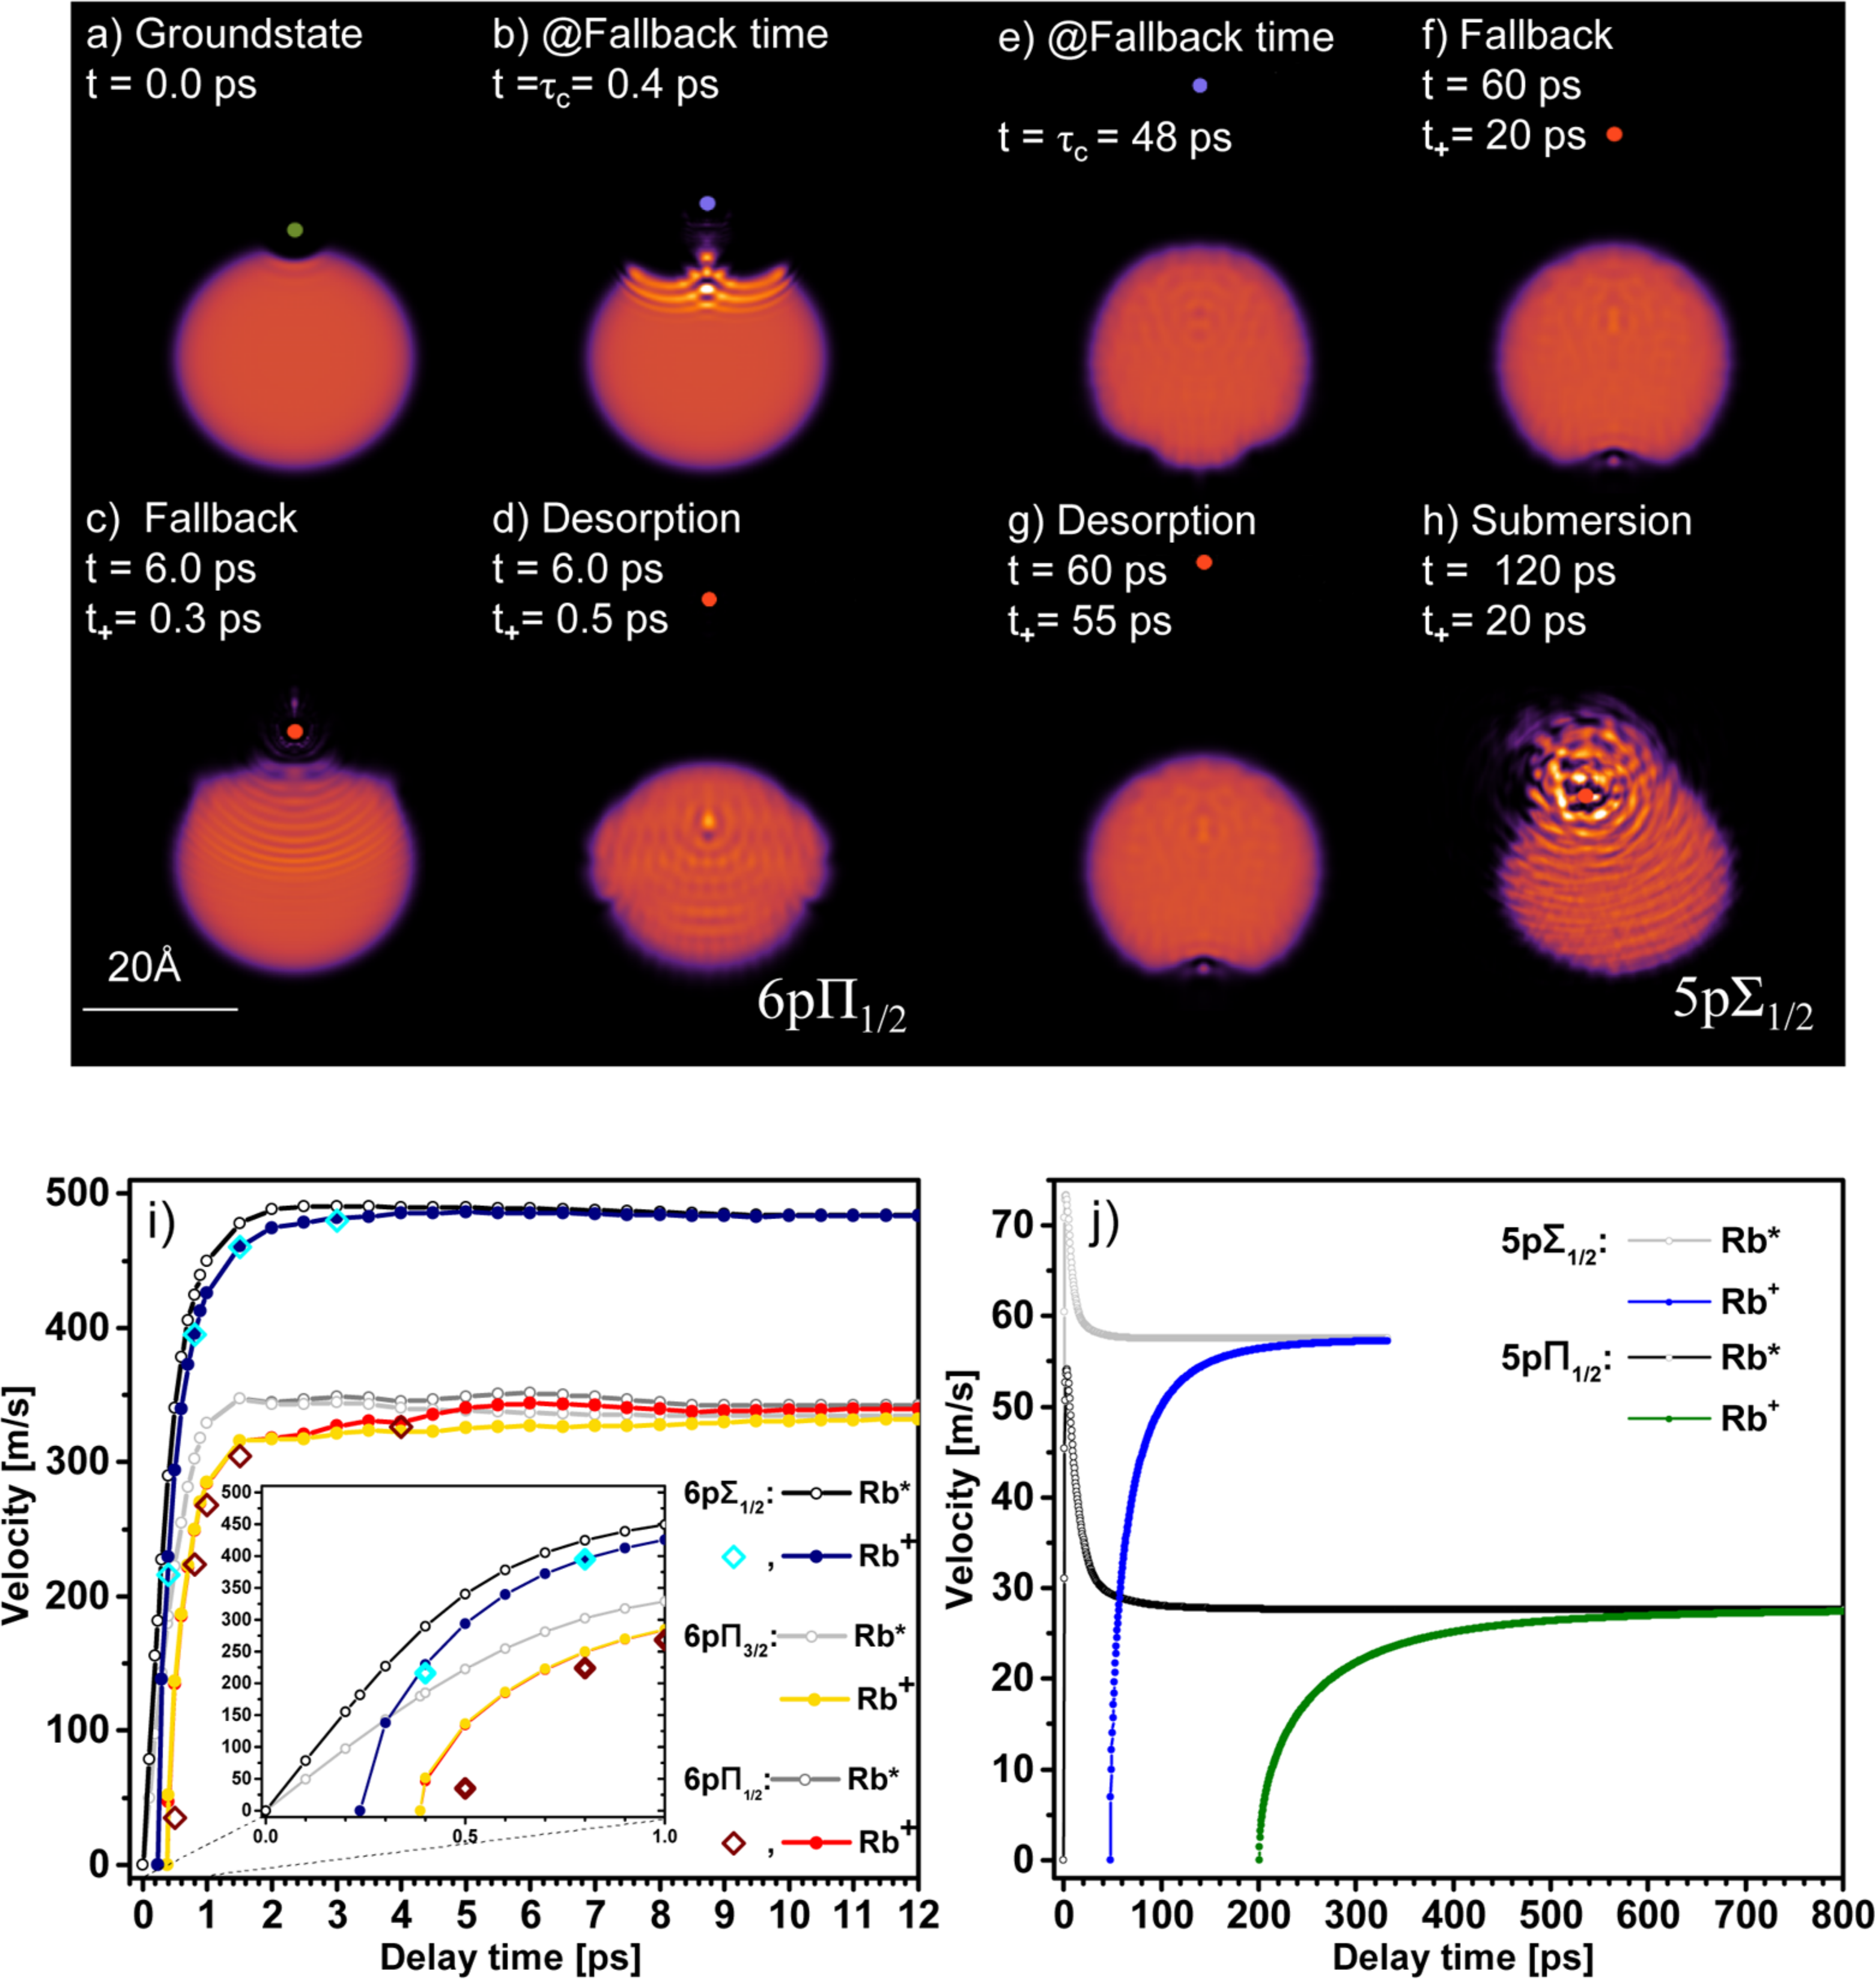
\includegraphics[width=\linewidth]{fallback-time}\label{fig:fallback-time}
			\caption{Densités 2D (a−d,e−h) et vitesses basées sur TDDFT (i,j) des atomes de Rb attaché à He$_{1000}$ excité de l'équilibre (a) à gouttelette perturbée états 6p (colonne de gauche) et 5p (colonne de droite). Les configurations sont affichées pour différents temps de propagation $t$ et les temps d'ionisation $t_+$ : (b,e) neutre Rb à \guillemotleft~fall-back time~\guillemotright{} $t=\tau_c$ ; (c,f) $t_+<\tau_c$, \guillemotleft~fall-back~\guillemotright{} de l'ion Rb$^+$ ; (d,g) $t_+>\tau_c$, désorption de Rb$^+$ ; (h) solvatation de Rb$^+$ ; (i,j) évolution des vitesses Rb* avec le temps $t$ (points ouverts gris), et vitesses finales de Rb$^+$ (points remplis de couleur) en fonction du $t_+$. (Voir Chapitre~\ref{ch:exc-state-dyn} de la thèse.)}
		\end{figure}		
		Dans l'article presenté dans Chapitre~4, une étude combinée expérimentale et théorique centrée sur l'imagerie et la caractérisation de la dynamique suivant les excitations 5p$\leftarrow$5s et 6p$\leftarrow$5s de rubidium hébergé par une nanogouttelette d'hélium. L'expérience a utilisé des techniques pompe-sonde femtoseconde avec un premier laser excitant le Rb sur la surface des gouttelettes au temps $t_{exc}$ et un second laser l'ionisant pour la détection avec VMI au temps $t_{ion}$. Les résultats ont caractérisé un délai critique, appelé \guillemotleft~fall-back time~\guillemotright, entre deux résultats opposés. Si $t_{ion}-t_{exc}\leq\tau$, l'atome Rb sortant est encore assez proche de la gouttelette lorsque le laser sonde rend son interaction attrayante. Par conséquent, le Rb$^+$ se retourne et est solvaté. D'autre part, pour $t_{ion}-t_{exc}\geq\tau$, l'ionisation se produit trop tard pour que Rb$^+$ ressente une attraction appréciable de la gouttelette, et il y avait déjà trop d'énergie cinétique pour qu'il s'échappe.
		
		L'étude théorique a porté sur la compréhension de la dynamique de désorption et la détermination des temps de repli à comparer avec l'expérience. Il a fait usage du He-TDDFT présenté dans \scn{sec:td-dft}, à la fois dans les états excités et ionisés. Les résultats sont présentés dans l'article suivant qui a été publié dans le Journal of Physical Chemistry Letters\citep{Vangerow2017}.
		
		Dans nos simulations, nous trouvons que les états excités au collecteur 5p et 6p désorbent à des échelles de temps très différentes, séparées par deux ordres de grandeur ($\sim$100~ps et $\sim$1~ps pour respectivement 5p et 6p). Ceci est en bon accord avec les résultats expérimentaux où le comportement de désorption des atomes de Rb photo-excités est déterminé en utilisant un schéma pompe-sonde femtoseconde.

	\section*{Dynamique de désorption des exciplexes RbHe\\\small(Chapitre~5)}
		\begin{figure}
			\centering
			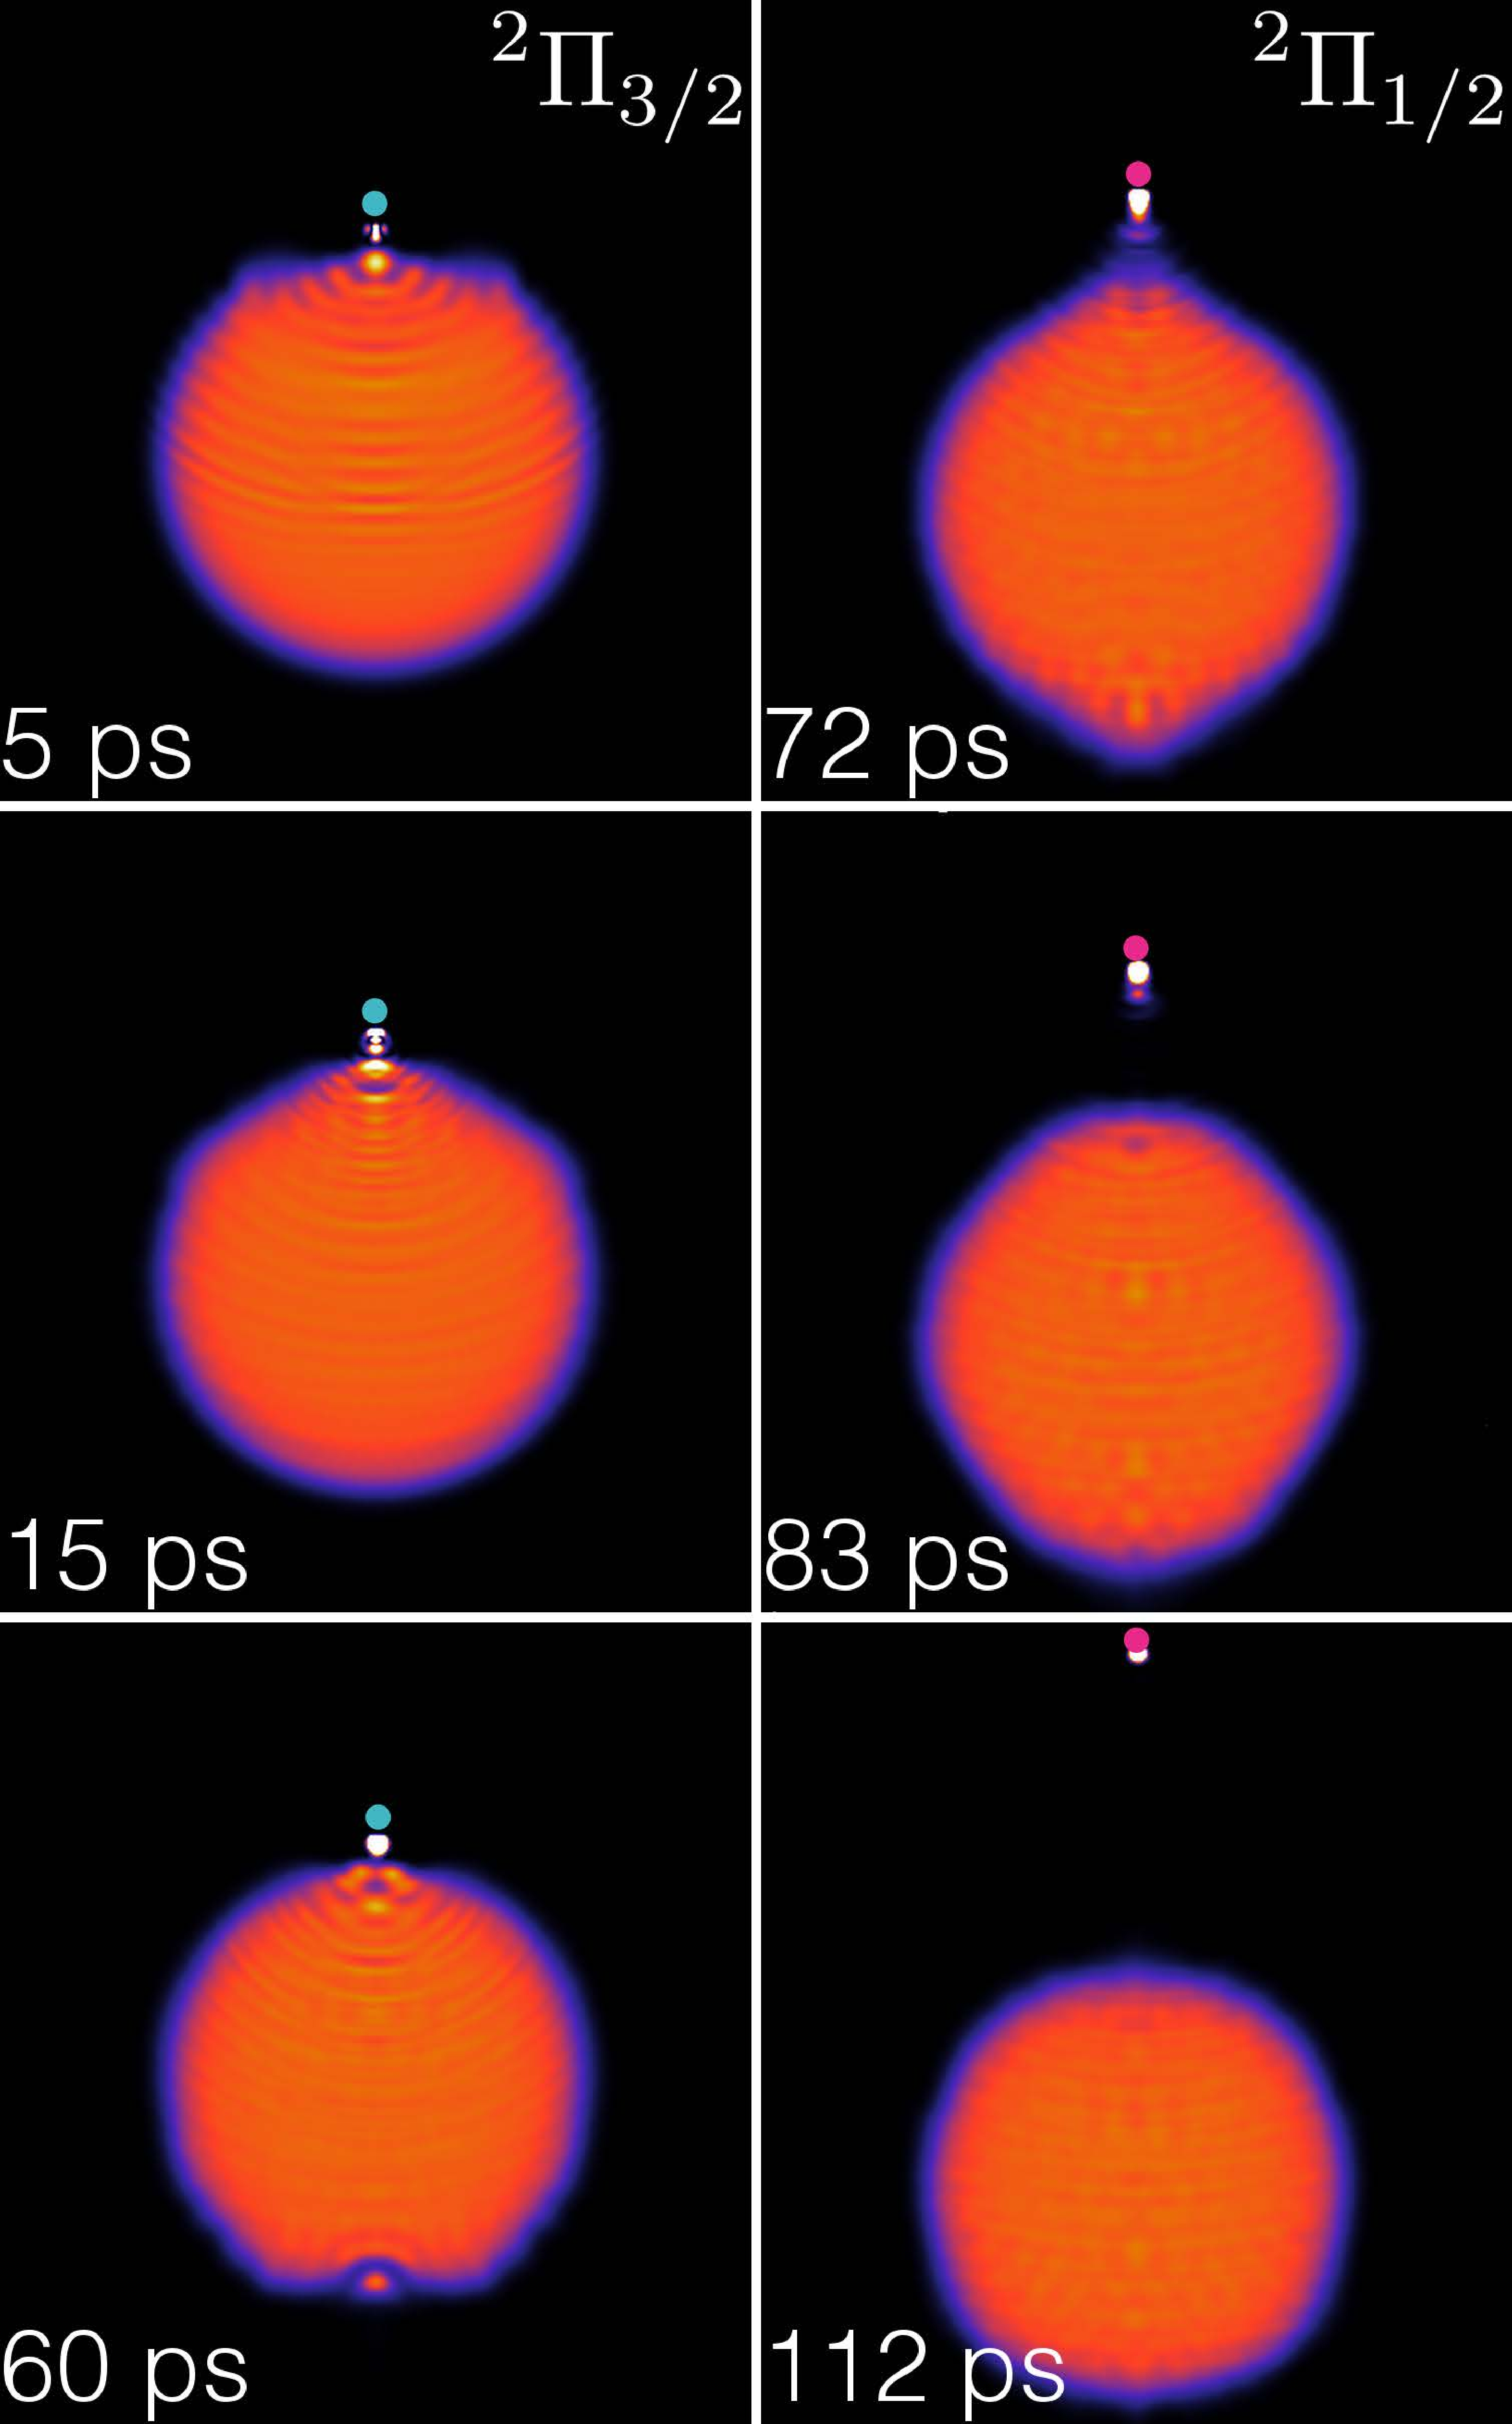
\includegraphics[width=0.9\linewidth]{fig5-pccp}\caption{Instantanés de la densité de l'hélium au cours de l'évolution du complexe RbHe$_{1000}$ excité pour $\eta$=15\%,~$\Delta t$=60~ps. Le point vert représente l'atome Rb, excité à l'état 5p$\Pi_{3/2}$ ; le point magenta est l'atome Rb après une relaxation soudaine à l'état 5p$\Pi_{1/2}$. (Voir Chapitre~\ref{ch:rbhe-exciplexe} de la thèse.)}
			\label{fig:snapshots}
		\end{figure}	
		Par contre, dans nos simulations, l'excitation à l'état 5p$\,^2\Pi_{3/2}$ aboutit à un exciplexe de RbHe lié à la surface, contrairement au cas expérimental où l'exciplexe RbHe désorbe des gouttelettes surface. En introduisant la relaxation de spin $^2\Pi_{1/2}\!\leftarrow\!^2\Pi_{3/2}$ dans les simulations, l'exciplex RbHe est capable de désorber à partir de la surface de la gouttelette, ce qui résout cette contradiction.
		
		Comment résoudre la divergence entre l'observation expérimentale que les atomes de Rb, excités à l'état 5p$\,^2\Pi_{3/2}$, se détachent de la surface des gouttelettes, et les simulations TD-DFT qui montrent qu'elles aboutissent à un état lié à la surface? C'est la question qui a conduit à ce travail. Lors de la photo-excitation de Rb à l'état 5p$\,^2\Pi_{3/2}$, un atome d'He peut y être attaché formant un exciplex HeRb; cela ne peut pas arriver si Rb est excité à l'état 5p$\,^2\Pi_{1/2}$ car il trouve une barrière (voir \fig{fig:potentials}) empêchant la formation d'exciplex.
		
		Dans la phase gazeuse, un exciplex HeRb~5p$\,^2\Pi_{1/2}$ peut être formé s'il y a assez d'énergie cinétique pour que Rb* surmonte la barrière de potentiel; alternativement, la collision d'HeRb~5p$\,^2\Pi_{3/2}$ exciplex avec un autre atome ou complexe pourrait relâcher l'atome Rb* de la 5p$\,^2\Pi_{3/2}$ à l'état 5p$\,^2\Pi_{1/2}$, surmontant la barrière car les puits potentiels pour les deux états sont à des distances Rb-He similaires. Dans la phase condensée (gouttelettes) à la température de 0.4~K, aucun de ces mécanismes n'est disponible pour expliquer la formation des exciplexes HeRb~5p$\,^2\Pi_{1/2}$ et leur éjection potentielle.
		
		Cependant, une autre possibilité pour cela est la désexcitation non radiative de 5p$\,^2\Pi_{3/2}$ vers les 5p$\,^2\Pi_{1/2}$ qui peuplent le dernier état et laisse l'atome Rb* avec assez d'énergie cinétique pour être éjecté. Notez dans la \fig{fig:potentials} que le minimum du potentiel 5p$\,^2\Pi_{3/2}$ est de 12683~cm$^{-1}$, et celui du 5p$\,^2\Pi_{1/2}$ potentiel est à 12518~cm$^{-1}$; la valeur de ce potentiel à la barrière est de 12611~cm$^{-1}$. Ainsi, une désexcitation non radiative de l'atome Rb* peut ajouter à son énergie cinétique d'origine jusqu'à 165~cm$^{-1}$. Il est à noter qu'il sera éjecté dans l'état 5p$\,^2\Pi_{1/2}$, et non dans le 5p$\,^2\Pi_{3/2}$ où il était précédemment photo-excité.
		
		Cette publication contient une extension de notre recherche expérimentale et théorique combinée présentée dans la section précédente. Nous nous intéressons ici à la formation de molécules de RbHe-exciplex libres à partir de nanoparticules d'He dopées au Rb et excitées par laser grâce au mécanisme de relaxation de spin électronique.

	\section*{Nanogouttelettes de potassium dopées\\\small(Chapitre~6)}
		Sous la supervision de Nadine Halberstadt et moi-même, un master de recherche de recherche ---\emph{M2 Physique Fondamentale}--- intitulé \emph{\textbf{\guillemotleft~Dynamique d'une nanogouttelette d'hélium superfluide dopée avec un seul atome de potassium~\guillemotright}} a été joué par Maxime Martinez.
		
		Le projet étudie le comportement statique et dynamique d'un seul atome de potassium (K) excité de la configuration d'équilibre K-$^4$He$_{1000}$ au K*(4p)-$^4$He$_{1000}$ et K*(5s)-$^4$He$_{1000}$ états. Le choix du potassium a été motivé par une discordance dans les études expérimentales résolues dans le temps\citep{Schulz2001,Reho2000-1,Reho2000-2}. De plus, la masse de potassium se situe entre celles des alcalis plus lourds comme le rubidium et le césium, et les plus légères, comme le lithium et le sodium. Par conséquent, le potassium présente un cas intéressant, étant à la limite entre le régime classique pour les alcalis lourds et un régime quantique pour les plus légers. Les deux traitements des propriétés d'équilibre et de l'excitation 5s $\leftarrow$ 4s sont étudiés. Ce travail n'est pas inclus dans cette thèse mais peut être trouvé dans\rf{Martinez2017}.
		
		On conclut que les effets quantiques de K existent mais ne sont pas essentiels à la compréhension et à la description de la dynamique. Donc l'excitation K*(4p)-$^4$He$_{1000}$ est étudiée avec une description classique de K.

	\section*{Tourbillons quantifiés en gouttelettes\\\small(Chapitre~7)}
		Le deuxième aspect concerne une investigation purement théorique inspirée des travaux récents de Gomez et Vilesov \emph{et al}., où les tourbillons quantifiés ont été visualisés en dopant des nanoparticules d'He avec des atomes d'argent, puis en les \guillemotleft~soft landing~\guillemotright{} sur un écran carbone. Les images au microscope électronique montrent de longs filaments d'amas d'atomes d'argent qui s'accumulent le long des noyaux des vortex. La formation de réseaux de tourbillons quantiques à l'intérieur de nanogouttelettes est également mise en évidence en utilisant l'imagerie par diffraction des rayons~X pour visualiser les motifs de Bragg caractéristiques des amas de xénon (Xe) piégés à l'intérieur des noyaux de vortex.
		
		L'une des signatures les plus claires de la nature quantique d'une substance - et en fait de la superfluidité - est l'apparition de vortex quantifiés. Contrairement à un fluide normal, qui tournera comme un corps solide lorsque son récipient se déplace à une faible vitesse angulaire, un superfluide restera au repos. Cependant, au-dessus d'une certaine vitesse angulaire critique, l'état thermodynamiquement stable d'un superfluide comprend un ou plusieurs vortex quantiques. Un tel vortex peut être caractérisé par une fonction d'onde macroscopique et une circulation de vitesse quantifiée en unités de $\kappa=\frac{h}{m}$, où $h$ est la constante de Planck et $m$ est la masse d'un atome $^4$He\citep{Don91,Pit03}. Récemment, l'étude de la vorticité a été étendue à des systèmes finis tels que les BEC confinés aux pièges\citep{Pit03,Fetter2009}. Le transfert d'énergie et de moment cinétique dans les systèmes finis entre les tourbillons quantifiés et les excitations de surface est particulièrement intéressant car il définit la dynamique de nucléation, la forme et la stabilité des vortex impliqués\citep{Pit03,Fetter2009}. En comparaison avec les BEC confinés, les gouttelettes $^4$He sont autonomes et présentent un cas pour le superfluide fortement interactif. De plus, le diamètre d'un noyau vortex d'environ 0,2 nm dans le superfluide $^4$He\citep{Don91} est petit par rapport à la taille des gouttelettes, suggérant une tridimensionnalité des vortex dans les gouttelettes. Le tourbillon en $^4$He gouttelettes a donc attiré un intérêt considérable\citep{Clo98,Lehmann2003,Bar06,Sti06}.
		
		Récemment, Gomez \emph{et al}. ont fait des expériences\citep{Gom12} où des tourbillons à l'intérieur des gouttelettes superfluides $^4$He, produites par l'expansion de l'hélium liquide, ont été tracés en introduisant des atomes d'Ag qui se groupaient le long des lignes de vortex dans les gouttelettes. Les gouttelettes d'hélium nécessaires à ce type d'expériences doivent être plus grandes qu'avant pour la spectroscopie atomique simple et les études de dynamique car elles doivent être suffisamment grandes pour pouvoir héberger une série de vortex dopés avec de nombreux agrégats d'Ag. Un schéma du principe expérimental est montré dans \fig{fig:vortex-machine}. Les gouttelettes d'hélium sont produites par expansion d'He, à 20 bars et à une température $T_0$=5.4-7~K, dans le vide à travers une buse. Les gouttelettes refroidissent rapidement par évaporation et atteignent une température de 0.37~K\citep{Hartmann1995}, ce qui est bien en dessous de la température de transition superfluide $T_\lambda=2.17\unit{K}$\citep{Don91,Pit03}. Plus loin en aval, les gouttelettes capturent 10 atomes de carbone dans un four\citep{Log11d}. Les gouttelettes sont ensuite abordées contre un substrat de film de carbone mince à température ambiante\citep{Log11d}. Lors de l'impact, les gouttelettes s'évaporent, laissant sur la surface les traces d'Ag, qui sont ensuite visualisées par un microscope électronique à transmission (TEM). La prévalence des dépôts allongés en forme de piste (voir \fig{fig:silver-filament}) montre que les tourbillons sont présents dans des gouttelettes de plus de 300~nm et que leur durée de vie dépasse quelques millisecondes.
		
		Deux ans plus tard Gomez \emph{et al}. rapporté\citep{Gom14} sur la formation de réseaux de vortex quantique à l'intérieur des gouttelettes. Ils ont utilisé l'imagerie par diffraction de rayons~X femtoseconde à une seule prise pour étudier la rotation de gouttelettes d'hélium-4 superfluides seules, isolées, contenant environ 10$^8$-10$^{11}$~atomes. La formation de réseaux de vortex quantique à l'intérieur des gouttelettes a été confirmée en observant les patrons de Bragg caractéristiques des amas de xénons piégés dans les noyaux des vortex (voir la \fig{fig:vortex-array}).
	
	\section*{Collisions frontales\\\small(Chapitre~8)}
		\begin{figure}
			\centerline{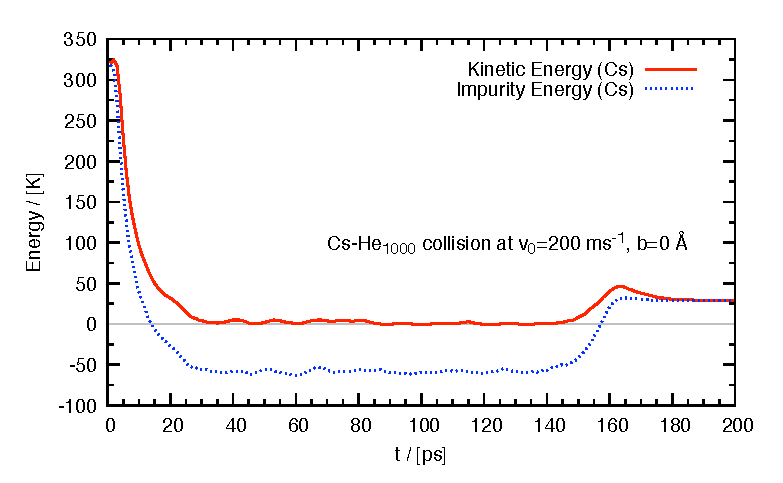
\includegraphics[width=\linewidth]{fig3-Cs-He}} 
			\centerline{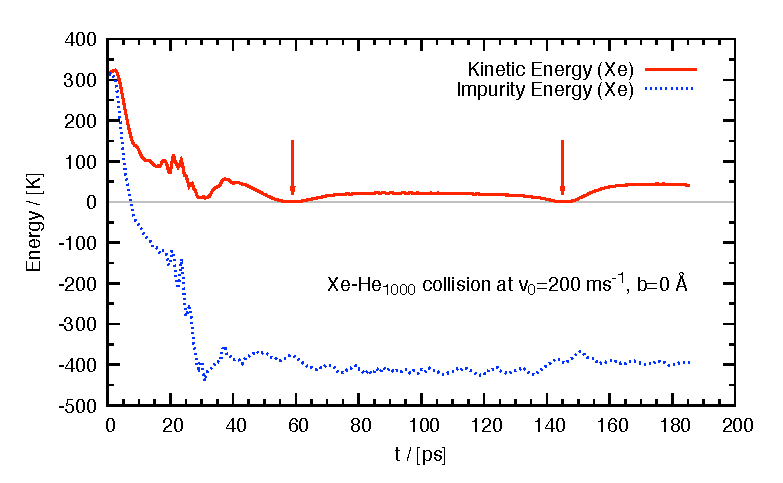
\includegraphics[width=\linewidth]{fig3-Xe-He}}
			\caption{\label{fig3-headon}Figure supérieure : Énergie cinétique et totale (cinétique et potentielle) en fonction du temps d'un atome de Cs, collision frontale contre une gouttelette de $^4$He$_{1000}$ à $v_0$=200~m/s. Figure inférieur : même que le figure supérieur pour un atome de Xe. Les flèches verticales indiquent les deux premiers points de virage à 59 et 145~ps, dont les densités d'hélium correspondantes sont indiquées dans la colonne de droite de la \fig{fig2-headon}.  (Voir Chapitre~\ref{ch:head-on-xece} de la thèse.)}
		\end{figure}	
		Motivés par des expériences récentes utilisant des atomes Xe pour visualiser des réseaux de vortex dans de très grandes gouttelettes d'hélium\citep{Gom14,Jon16}, nous présentons ici un premier pas vers la description de la capture d'atomes de Xe par des gouttelettes d'hélium, à savoir Xe atomes contre une gouttelette $^4$He$_{1000}$. Une discussion sur la capture dynamique des atomes de Xe par des gouttelettes hébergeant des vortex ligne et des tableaux vortex sera fournie par une prochaine étude combinant la simulation DFT des réseaux vortex comme dans\rfs{Anc14,Anc15} pour les nanocylindres et nanogouttelettes d'hélium et la collision avec les atomes de Xe dans ce travail. Dans la mesure du possible, les résultats pour Xe, un atome héliophile, sont mis en contraste avec les résultats pour Cs, un atome héliophobe de masse similaire.
		
		Nous considérons une gouttelette faite de $N=1000$ atomes d'hélium. Sa structure d'état fondamental est obtenue en utilisant DFT et donne un rayon de densité d'environ 22.2~\AA. Ensuite, la dynamique est initiée en plaçant l'atome Xe 32~\AA{} à l'écart du centre de masse (COM) de la gouttelette avec un paramètre d'impact égal à zéro (collision frontale). Les simulations sont effectuées pour des vitesses Xe initiales $v_0$ allant de 200 à 600~m/s dans le système de référence de la gouttelette, correspondant à des énergies cinétiques comprises entre 315.8~K et 2842~K. Ces énergies peuvent être comparées à l'énergie de solvatation d'un atome de Xe au centre d'une gouttelette $^4$He$_{1000}$, $S_{{\rm Xe}}=E({\rm Xe}@^4{\rm He}_{1000})-E(^4{\rm He}_{1000})=-$316.3~K. Par souci de comparaison, l'énergie de solvatation de Cs est de -5.2~K et sa position d'équilibre est dans une fossette à la surface extérieure des gouttelettes, environ 26.6~\AA{} de son centre.
		
		Les atomes thermiques Xe ($v_0\!\!\sim$240~m/s) sont utilisés dans les expériences\citep{Gom14,Jon16}, et la vitesse moyenne des gouttelettes est d'environ 170~m/s\citep{Gom11}.
		
		Nous montrons que les collisions frontales de nanogouttelettes d'hélium avec du xénon, un atome héliophile, impliquent un échange d'énergie cinétique du même ordre de grandeur que le césium, un atome héliophobe de masse similaire. Dans les deux cas, cette énergie est largement dissipée en produisant des ondes énergétiques dans la gouttelette ou elle est emportée par des atomes d'hélium rapidement émis. La différence entre les deux atomes est due à la nature différente de leur interaction avec l'hélium. Une accumulation de densité est observée autour du xénon héliophile lors de la dynamique, alors qu'une bulle est créée autour du césium héliophobe. Il faut donc beaucoup plus de vitesse pour que le xénon traverse la gouttelette et s'échappe que pour le césium, comme on pouvait s'y attendre.
	
	\section*{Capture par He gouttelettes\\\small(Chapitre~9)}
		Récemment, une technique a été introduite pour déterminer la taille des grosses gouttelettes d'He ($N>10^5$). Elle est basée sur l'atténuation d'un faisceau continu de gouttelettes par des collisions avec des atomes d'Ar à température ambiante\citep{Gom11}. La chambre de prélèvement de l'appareil à faisceau de gouttelettes est remplie de gaz argon et les gouttelettes d'hélium subissent de multiples collisions isotropes avec les atomes Ar sur leur chemin vers la chambre de détection.
		
		De grosses gouttelettes d'hélium pourraient également être dopées de cette manière. Cette méthode, utilisant des atomes Xe, a été instrumentale pour la détection et l'imagerie des réseaux de vortex quantifiés dans les gouttelettes d'hélium\citep{Gom14,Jones2016}. Des atomes Xe ont été utilisés dans ces expériences en raison de leur grande sensibilité à l'imagerie par diffraction cohérente aux rayons~X utilisée pour les détecter dans les gouttelettes d'hélium. Des expériences avec de grandes gouttelettes d'hélium superfluides sont passées en revue dans une publication récente\citep{Tan17}.
		
		L'interaction impureté-gouttelette en présence de vortex est également pertinente en tant que première étape d'un processus plus complexe conduisant à la formation de nanofils, voir par exemple\rfs{Lebedev2011,Gom12,Lat14,Tha14}. Des filaments longs constitués de particules d'hydrogène solides de taille micrométrique piégées sur des noyaux vortex quantifiés ont été utilisés pour imager directement la reconnexion vortex entre les vortex quantifiés dans l'hélium superfluide\citep{Bewley2008}.
		
		Ici nous présentons les résultats obtenus dans TDDFT pour la collision et la capture des atomes Xe et Ar par une gouttelette $^4$He$_{1000}$ à différentes énergies cinétiques et paramètres d'impact. Une attention particulière est accordée à l'interaction dépendante du temps des atomes de Xe et Ar avec des nanogouttelettes d'hélium contenant des lignes de vortex, et à l'effet de réseaux de tourbillons dopés à plusieurs couches dans de grosses gouttelettes d'hélium.
		
		En raison du coût de calcul élevé des simulations TDDFT présentées ici, nous abordons seulement quelques facettes du processus de capture que nous considérons comme pertinentes expérimentalement plutôt que d'effectuer une étude systématique du processus. En particulier:
		\begin{itemize}
			\item Nous étudions la capture d'atomes de Xe par une nanogoutte de $^4$He, à la fois pour des collisions frontales et pour différents paramètres d'impact, avec des vitesses de valeurs thermiques allant jusqu'à plusieurs centaines de m / s. Les résultats des collisions périphériques avec différentes valeurs du paramètre d'impact sont utilisés pour estimer la section efficace pour la capture Xe.
			\item Nous étudions comment un atome Xe interagit dynamiquement avec une gouttelette hébergeant une ligne de vortex, dans différentes conditions initiales résultant en différents régimes de vitesse de l'impureté lorsqu'il entre en collision avec le noyau vortex:
			\begin{enumerate}
				\item[i)] un atome Xe initialement au repos sur la surface des gouttelettes et s'enfonçant sous l'effet des forces de solvatation;
				\item[ii)] une collision frontale d'un atome Xe ou Ar en mouvement contre la nanogouttelette de $^4$He.
			\end{enumerate}
			\item Nous étudions l'état stationnaire d'une grosse gouttelette de $^4$He$_{15000}$ contenant un anneau de six lignes de vortex, dopées avec des atomes d'Ar remplissant complètement les six noyaux de vortex. C'est le système le plus simple qui imite ceux décrits expérimentalement dans\rf{Gom14}, où des réseaux de vortex dopés incorporés dans des microgouttes rotatives $^4$He ont été imagés.
		\end{itemize}

		\subsection*{Capture par des gouttelettes sans vortex}
			Nous avons simulé des collisions frontales d'un atome Xe avec une gouttelette $^4$He$_{1000}$ à des vitesses relatives $v_0$ allant de 200 à 600~m/s. La \fig{fig1-capture} affiche les diagrammes en deux dimensions de la densité d'hélium pour la valeur la plus élevée, $v_0\!=$600~m/s. Cette vitesse est bien au-dessus de la plage de vélocité typiquement rencontrée dans les expériences\citep{Gom11,Gom14,Jones2016}. Malgré l'apparition d'une densité d'hélium déconnectée dans le cadre $t$=87~ps, nous avons découvert que l'atome Xe tourne finalement et est à nouveau capturé à l'intérieur de la gouttelette même à cette vitesse d'impact relativement élevée. Notez que l'impureté Xe, même lorsqu'elle émerge temporairement de la masse de la gouttelette, semble être recouverte de quelques atomes de $^4$He, voir la configuration à 87~ps.

		\subsection*{Tourbillons de ligne}
			Pour déterminer la structure d'une gouttelette hébergeant un tourbillon linéaire singulièrement quantifié, nous avons commencé l'itération temporelle imaginaire à partir d'une densité d'hélium dans laquelle le tourbillon est \guillemotleft~imprimé~\guillemotright. A cet effet, une ligne de vortex le long de $z$ peut être décrite par la fonction d'onde effective 
			\begin{equation}
				\Psi_0(\mathbf{r}) = \rho_0^{1/2}(r)\,\mathrm{e}^{i\,{\mathcal S}(\mathbf{r})} = \rho_0^{1/2}(\mathbf{r}) \, \frac{(x + i y)}{\sqrt{x^2 + y^2}} \label{eq11-sum}
			\end{equation}
			où $\rho_0(\mathbf{r})$ est la densité de la gouttelette pure ou impureté dopée sans vortex. Les lignes de vortex le long d'autres directions passant par un point choisi peuvent également être imprimées\citep{Pi07}.

			Dans le cas représenté par l'\eq{eq11-sum}, si l'impureté est dans le vortex le long d'un axe de symétrie du complexe impureté-gouttelette, la fonction d'onde effective $\Psi_0({\mathbf r})$ ---avant et après relaxation--- est un vecteur propre de l'opérateur de moment angulaire $\hat{L}_z=-i\,\hbar\partial/\partial\theta$.
			Le moment angulaire de la gouttelette est alors
			\begin{equation}
				\langle \hat{L}_z \rangle = \langle \Psi_0(\mathbf{r}) | \hat{L}_z | \Psi_0(\mathbf{r}) \rangle = N \; \hbar
				\label{eq12-sum}
			\end{equation}

	\subsection*{Capturer la dynamique par les tourbillons}
		\begin{figure}
			\centering
			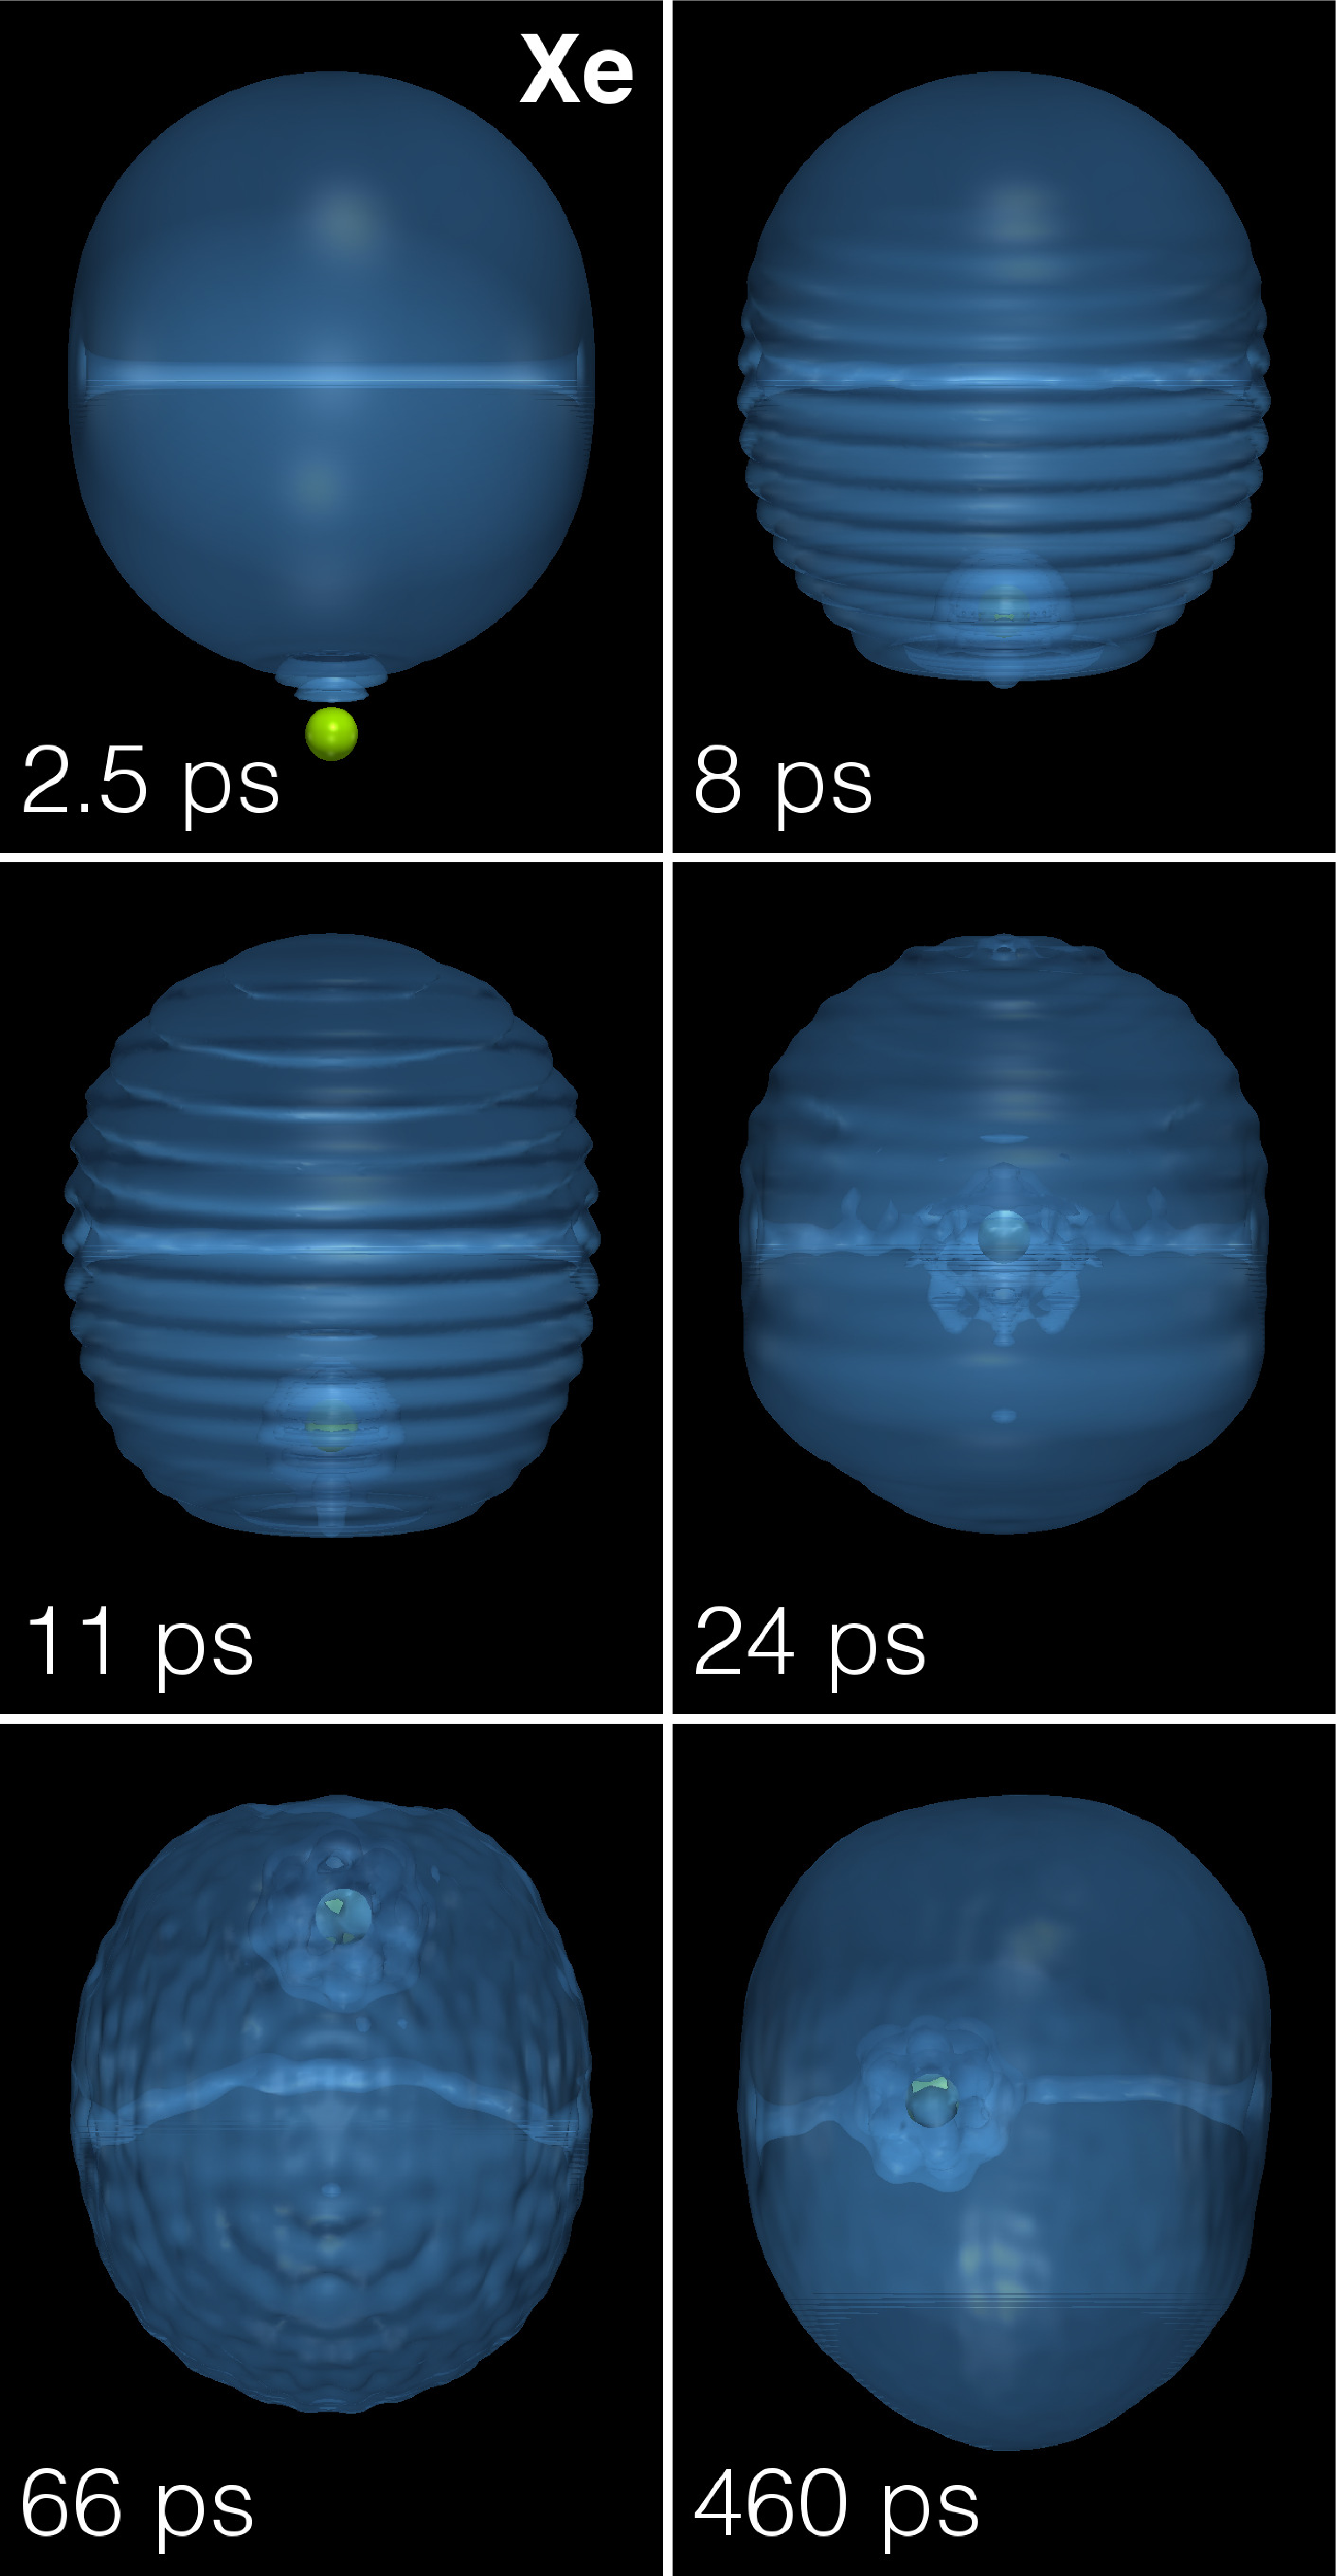
\includegraphics[width=0.75\linewidth]{fig10}
			\caption{\label{fig10-capture}
			Evolution dynamique d'un atome de Xe (point vert) approchant une gouttelette de $^4$He$_{1000}$ hébergeant une ligne de vortex par dessous à $v_0$=200~m/s. L'heure correspondante est indiquée dans chaque image. (Voir Chapitre~\ref{ch:capture} de la thèse.)}
		\end{figure}	
		Pour étudier l'interaction d'une impureté atomique avec des vortex, nous avons imprimé une ligne de vortex dans la gouttelette $^4$He$_{1000}$ et préparé l'atome Xe dans différentes conditions cinématiques.

La diffusion inélastique d'atomes de xénon par des vortex quantifiés dans de l'hélium en vrac superfluide a été traitée dans\rf{Psh16}.
 Il s'est avéré qu'une collision frontale conduit à la capture de Xe par la ligne de vortex pour $v_0$=15.4~m/s, mais pas pour $v_0$=23.7~m/s.
Nous avons effectué une simulation équivalente en plaçant initialement
 l'atome Xe à l'intérieur de la gouttelette 10~\AA{} de la ligne de vortex et l'envoyant de front vers le vortex à une vitesse de 10~m/s.
Cette vitesse est de l'ordre de la vitesse thermique d'un atome Xe dans une gouttelette dans des conditions expérimentales,
une fois que la gouttelette s'est thermalisée après avoir capturé l'atome Xe ($T\!\!\sim$0.4~K)\citep{Toe04}.
Puisque la position d'équilibre de l'atome Xe est au centre de la gouttelette, elle se déplace vers cette région et y reste pendant le reste de la simulation.
Dans cette région de la gouttelette, l'atome Xe est également attiré par le vortex, mais il est dévié par l'écoulement superfluide autour de la ligne de vortex et finit par tourner autour de lui.
 Par conséquent, il est capturé par le vortex sans entrer dans son noyau.
 
 	\subsection*{Tableaux de vortex en gouttelettes}
L'existence de réseaux de vortex ordonnés à l'intérieur des gouttelettes $^4$He a été établie par l'apparition de motifs de Bragg
Clusters Xe piégés à l'intérieur des noyaux de vortex dans des gouttelettes faites de $N$=10$^8$-10$^{11}$ atomes
(correspondant à des rayons de 100 à 1000 nm)\citep{Gom14,Jones2016}. Nous avons récemment étudié la stabilité du vortex
tableaux de jusqu'à $n_v$=9 vortices
à l'intérieur d'une nanogouttelette $^4$He en utilisant l'approche DFT\citep{Anc15}.
Il s'est avéré que
la structure favorisée énergiquement pour $n_v\!\!>$6 est un anneau
de vortex encerclant un vortex au centre de la gouttelette.
Fot $n_v$=6, la configuration avec un anneau de six vortex se trouvé pour avoir presque
la même énergie que l'anneau à cinq plis
plus un vortex au centre. L'ancienne structure
a été observée expérimentalement\citep{Gom14,Jones2016,Ber17},
bien que la théorie du vortex classique
prédit pour elle un coût d'énergie libre beaucoup plus élevé que pour le dernier\citep{Cam79}.
Des structures d'équilibre similaires ont été obtenues au sein de DFT pour
nanocylindres d'hélium hébergeant des baies de vortex\citep{Anc14}.

Nous avons cherché des configurations stationnaires d'un anneau à 6 vortex
dans une gouttelette tournante He$_{15000}$ en résolvant
Les équations EL dans le cadre corotant avec un fixe
vitesse angulaire. Chaque noyau de vortex est rempli avec des atomes d'Ar
atomes, et le système est autorisé à se détendre complètement.
En fin de compte, la colonne d'atomes à l'intérieur de chaque noyau de vortex atteint une structure d'équilibre
où les atomes Ar sont séparés d'une distance qui est à peu près celle du dimère Ar.
Une telle configuration est montrée dans \fig{fig13-capture}. Notez que
les noyaux des vortex sont presque des lignes droites, alors que dans un
gouttelette non dopée tournant avec la même vitesse
les lignes de vortex seraient courbées,
comme montré par exemple dans \fig{fig7-capture}.
Les atomes Ar ne sont pas représentés sur la figure.
Les structures localisées apparaissant dans les noyaux de vortex sont des régions haute inhomogène, haute densité de $^4$He
résultant du potentiel attractif Ar-He.

Nous montrons que les atomes Xe et Ar à des vitesses thermiques sont facilement capturés par des gouttelettes d'hélium, avec une coupe transversale de capture similaire à la section transversale géométrique de la gouttelette. Essentiellement pour la capture subséquente d'impuretés par des lignes de vortex, nous avons également montré que la plus grande partie de l'énergie cinétique de l'impureté est perdue dans le processus de capture pendant les premières dizaines de picosecondes. Cela se produit soit par l'éjection d'atomes He promptement émis, soit par la production d'ondes sonores et de grandes déformations dans la gouttelette.

En outre, nous avons également montré que si la gouttelette héberge un vortex, les impuretés, se déplaçant lentement, sont facilement capturées par la ligne de vortex. Plutôt que d'être piégée à l'intérieur du noyau du vortex, l'impureté doit se déplacer à une distance proche de celle-ci. Outre la perte d'énergie cruciale lorsque l'impureté frappe la gouttelette, la capture par le vortex est favorisée par un transfert d'énergie supplémentaire de l'impureté à la gouttelette: des déplacements de grande amplitude de la ligne de vortex ---comme indiqué dans le ESI\citep{ESI}--- ont lieu, constituant une autre source de la perte d'énergie cinétique dans les dernières étapes de la capture. Un problème connexe est l'apparition de modes Kelvin dans la ligne de vortex, qui n'est pas seulement courbée, mais aussi tordue au cours de la collision.

Nous pouvons conclure que si les conditions cinématiques de la collision (énergie cinétique et paramètre d'impact) conduisent à la capture de l'impureté par la gouttelette, l'effet de flipper provoqué par la surface des gouttelettes peut faciliter la rencontre de l'atome Xe/Ar et du vortex ligne ---et la capture possible de l'atome par le vortex--- puisque les deux ont tendance à rester dans la région interne de la gouttelette. Nous l'avons montré dans le cas de Xe à $v_0$=200~m/s : Xe est capturé lors de son deuxième transit à travers la gouttelette, alors que cela ne pourrait pas se produire dans l'hélium liquide\citep{Psh16}. Cet effet pourrait expliquer la capture d'impuretés par des lignes de vortex même dans les très grosses gouttelettes utilisées dans l'observation de nanostructures en forme de filaments.

	\section*{Perspectives d'avenir}
		Notre travail sur la dynamique en temps réel de la photo-excitation d'un atome de métal alcalin sur la surface d'une nanogouttelette d'hélium est assez vaste. Mener le même type d'études sur d'autres types d'espèces dopantes qui sont solvatées plus profondément à l'intérieur des gouttelettes He (par exemple métaux alcalino-terreux, métaux de transition) permettrait de mieux comprendre les mécanismes de désolvatation et d'éjection des atomes d'impuretés excités\citep{Loginov:2007,Loginov:2012,Kautsch:2013,Lindebner:2014}.
		
		De plus, une description plus complète des couplages entre les états électroniques et les degrés de liberté de configuration dans de tels complexes excités induits par l'environnement des gouttelettes He serait hautement souhaitable\citep{Closser:2014,Masson:2014}. Dans une avancée récente, la relaxation électronique des cations Ba$^+$ dans les nanogouttelettes He, basée sur une diabatisation des potentiels d'interaction des états électroniques excités par He-Ba$^+$ et par les états excités\citep{Vindel:2018}, a été proposée comme un mécanisme pour éjecter Ba$^+$ et {Ba$^+$He$_n$} des gouttelettes He. Ces mécanismes de relaxation de spin et de relaxation d'état inter-électronique doivent être confirmés par des études de dynamique en temps réel.
		
		Enfin, les capacités de l'approche He-DFT pourraient aider à élucider des processus d'intérêt expérimental, comme la capture d'une ou plusieurs impuretés par de grosses gouttelettes hébergeant un réseau de vortex; et comment plusieurs impuretés atomiques, touchant une gouttelette en rotation hébergeant des vortex, réagissent en formant de petites grappes, finalement piégés à l'intérieur des noyaux de vortex, comme indiqué par l'apparition de nanostructures en forme de filament dans des expériences.

		Dans toutes ces futures lignes de recherche, $^4$He-DFT et TDDFT seront des outils essentiels, étant donné leur capacité à décrire avec précision les propriétés d'équilibre et de dynamique des nanogouttelettes d'hélium de taille réaliste, pouvant accueillir des tourbillons, en interaction avec des dopants. Dans ce contexte, il sera extrêmement intéressant de coupler $^4$He-TDDFT avec la dynamique moléculaire quantique pour aller au-delà de l'approximation du champ moyen de la dynamique du dopant dans l'environnement de l'hélium. Une alternative prometteuse dans l'approche de la fonction de base corrélée (CBF) et son approche multi-composantes récemment développée par Rader \textit{et al.}\Citep {Rader2017}
		
		\vspace{25ex}
		\filleft{\bfseries\itshape\fontsize{50}{60}\selectfont\textcolor{activeColor}{Fin}}